\section{Deeltjesproductie}

%%%%%%%%
\subsection{Vierimpuls}

% \begin{figure} [h]
% \begin{center}
% \mbox{\epsfxsize=12cm\epsffile{oefeningen.pictures/productie.eps}}
% \caption{}
% \label{f:productie}
% \end{center}
% \end{figure}

\begin{figure}[ht]
\centering
\includegraphics[width=.8\textwidth]{oefeningen.pictures/productie}
\caption{}
\label{f:productie}
\end{figure}

Een deeltje met massa $m$ botst op een zelfde deeltje in 
rust (fig. \ref{f:productie}a).
\begin{itemize}
\item [a.]
Wat is de vierimpuls van een ieder van de deeltjes?
\item [b.]
Wat is de norm van ieder van deze vierimpulsen?
\item [c.]
Wat is de totale vierimpuls in het laboratoriumsysteem?
\end{itemize}
Beschouw nu de botsing in het zwaartepuntsysteem (fig. \ref{f:productie}b).
\begin{itemize}
\item [d.]
Wat is de totale vierimpuls in het zwaartepunt systeem?
\item [e.]
Wat is de norm van deze vierimpuls?
\item [f.]
Vind de uitdrukking voor $E$ in termen van $E^{*}$ en $m$.
\end{itemize}

\subsection{$p\vec{p}$ botsing}
In het zwaartepuntsysteem botsten een
proton (symbool $p$) en een antiproton (symbool $\bar{p}$) ieder met een
snelheid $v= 0,8c$ op elkaar.
De massa van het antiproton is gelijk aan de massa van het proton.
\begin{itemize}
\item [a.]
Wat is de totale impuls $p^{*}$ in het zwaartepuntsysteen?
\item [b.]
Wat is de totale energie $E^{*}$ in het zwaartepuntsysteem?
\item [c.]
Wat is de totale vierimpuls $P^{*}$ in het zwaartepuntsysteem?
\item [d.]
Bij de botsing vernietigen de twee deeltjes elkaar.
Hoeveel energie is er beschikbaar voor de creatie van nieuwe
deeltjes?
\end{itemize}

%%%%%%%%%%%%%
\subsection{Vervallende deeltjes}
Een deeltje in rust met massa $M$ vervalt in twee identieke deeltjes, elk 
met massa $m$.
\begin{itemize}
\item [a.]
Waarom zullen de twee deeltjes die ontstaan een even grote snelheid hebben?
\item [b.]
Geef een uitdrukking voor deze snelheid $v$ in termen van
$M$ en $m$.
\end{itemize}
Een pion (massa $m_{\pi})$ in rust vervalt in een muon (massa $m_{\mu})$ en een
neutrino (massa $m_{\nu} = 0$).
\begin{itemize}
\item [c.]
Wat is de snelheid van het neutrino?
\item [d.]
Wat is de impuls van het muon?
\end{itemize}

%%%%%%%%%%%
\subsection{$pp$ botsing}

% \begin{figure} [h]
% \begin{center}
% \mbox{\epsfxsize=12cm\epsffile{oefeningen.pictures/ppbotsing.eps}}
% \caption{pp botsing}
% \label{f:ppbotsing}
% \end{center}
% \end{figure}

\begin{figure}[ht]
\centering
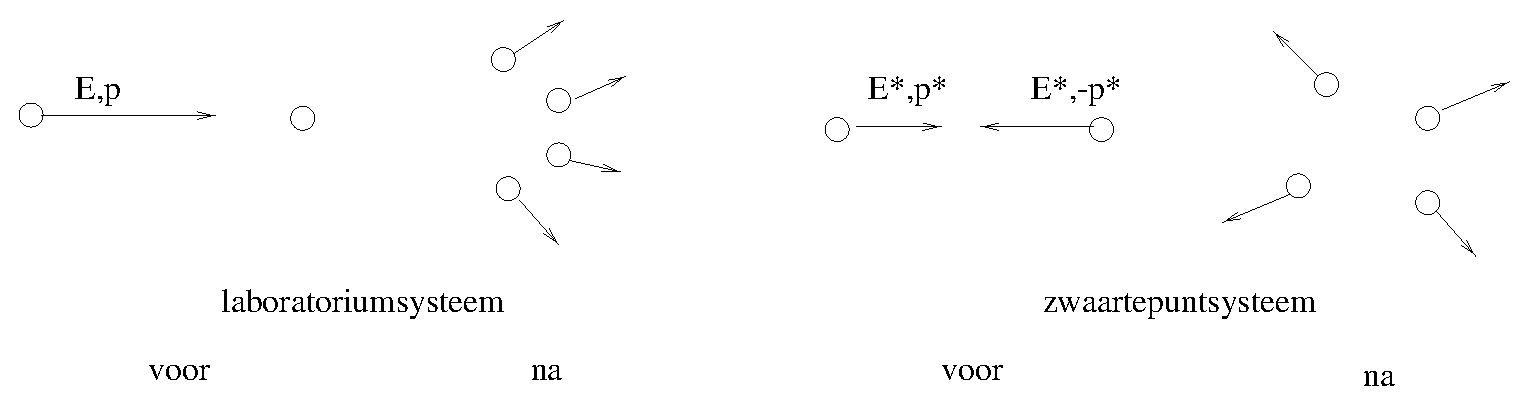
\includegraphics[width=.8\textwidth]{oefeningen.pictures/ppbotsing}
\caption{pp botsing}
\label{f:ppbotsing}
\end{figure}

Wanneer een proton met voldoende energie op een andere proton wordt
geschoten is het mogelijk dat een extra $p\bar{p}$ paar wordt gecre\"{e}erd:
$pp \rightarrow ppp\bar{p}$ 

Bekijk de gebeurtenis eerst vanuit het laboratoriumsysteem
(figuur \ref{f:ppbotsing} links).
De energie en impuls van het bewegende proton in het laboratoriumsysteem 
zijn resp. $E$ en $p$.
\begin{itemize}
\item [a.]
Welk verband bestaat er tussen $E$ en $p$?
\item [b.]
Wat is de totale energie in het laboratoriumsysteem v\'{o}\'{o}r de botsing? 
En de totale impuls? 
\item [c.]
Bekijk nu de gebeurtenis in het zwaartepuntsysteem
(figuur \ref{f:ppbotsing} rechts).
Wat is de minimale energie ($E^{*}_{min}$) nodig om de 
reactie $pp \rightarrow ppp\bar{p}$
te laten verlopen?
\item [d]
Leid uit de invariantie van de vierimpuls de waarde voor de minimale 
energie $E_{min}$ af.
\item [e.]
Wat zou energetisch voordeliger zijn: 
de hierboven beschreven botsing met \'{e}\'{e}n bewegend
en \'{e}\'{e}n stilstaand proton of de situatie waarbij twee bewegende 
protonen op elkaar botsen (bij gelijke onderlinge snelheid)?
\end{itemize}

%%%%%%%%%%%%%%
\subsection{Eenheden}
De energie-eenheden eV (elektronvolt), MeV, GeV, enz., kunnen ook gebruikt 
worden om massa en impuls in uit te drukken: de massa van een electron 
is ongeveer  $m_{e}=0,5$ MeV/c$^{2}$.
\begin{itemize}
\item [a.]
Hoe groot zijn dan $\gamma$  en $v$ voor een elektron met energie  
$E=1$ MeV? 
\item [b.]
Hoe groot is zijn impuls? Welke eenheid gebruik je dan?
\item [c]
De massa van een proton is  $m_{p}=1,0$ GeV/$c^2$ .
Hoeveel energie en impuls heeft een proton met snelheid  $v=0,8\ $ $c$?
\end{itemize}

%%%%%%%%%%%%%
\subsection{$e^{-}e^{+}$ botsing}
Een elektron botst in het laboratoriumsysteem met snelheid $v = 0,8c$ op een
positron in rust.
\begin{itemize}
\item [a.]
Bereken hun totale energie in het laboratoriumsysteen 
($E_{tot} = E_{e^{-}} + E_{e^{+}}$) uitgedrukt in 
de elektron massa $m_{e}$.
\item [b.]
Dezelfde vraag in het zwaartepuntssysteem ($E^{*}_{tot} = E^{*}_{e^{-}} + E^{*}_{e^{+}}$).
\end{itemize}
Bij de botsing vernietigen zij elkaar en ontstaan er, gezien vanuit het 
zwaartepuntsysteem, twee gelijke fotonen die tegengesteld aan elkaar 
wegschieten, elk met een energie $E^{*}_{foton} = h \nu$.
\begin{itemize}
\item [c.]
Waarom moeten het twee fotonen zijn en waarom hebben ze dezelfde frequentie?
\end{itemize}
Als de beweging van de fotonen in het zwaartepuntsysteem loodrecht 
op de richting van het elektron is, kun je met een Lorentztransformatie
de energie van de fotonen in het laboratoriumsysteem bepalen.
\begin{itemize}
\item [d.]
Wat is de frequentie van de fotonen in het laboratoriumsysteem?
\end{itemize}
